\input{../YKY-preamble}

\newcommand{\ovalA}{\; \vcenter{\hbox{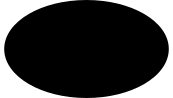
\includegraphics[decodearray={0.4 1 1.0 1 0.4 1}]{../oval.png}}} \;}
\newcommand{\ovalB}{\; \vcenter{\hbox{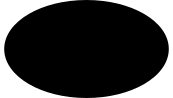
\includegraphics[decodearray={1.0 1 0.4 1 0.4 1}]{../oval.png}}} \;}
\newcommand{\ovalC}{\; \vcenter{\hbox{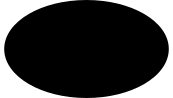
\includegraphics[decodearray={0.9 1 0.8 1 0.4 1}]{../oval.png}}} \;}


\title{Learning inside the Rete algorithm}

\author{YKY (Yan King Yin) \\ {\footnotesize general.intelligence@gmail.com}}

\begin{document}

	\setlength{\parindent}{0pt}
	\setlength{\parskip}{2.8ex plus0.8ex minus0.8ex}
	
	\maketitle
	
\begin{abstract}
\end{abstract}

\section{Introduction to the Rete algorithm}

The general form of a \textbf{production rule} is like this:
\begin{equation}
\overbrace{\ovalA \wedge \ovalA \wedge \ovalA ....}^{\mbox{condition}} \rightarrow \overbrace{\ovalB}^{\mbox{action}}
\end{equation}
where $\wedge$ denotes logical conjunction (AND).

Typically, we would be trying to match a relatively small number of \textbf{facts} (that represent the current \textbf{state}, or \textbf{working memory}) against a very large number of \textbf{rules}:
\begin{equation}
\overbrace{\scalebox{0.7}{\parbox{9em}{.... $\ovalC \ovalC \ovalC$}}}^{\mbox{queue of WMEs}} \quad \mbox{ match against } \quad
\scalebox{0.7}{\parbox{0.3\linewidth}{
\begin{align}
\ovalA \ovalA \ovalA .... \rightarrow \ovalB \nonumber \\
\ovalA \ovalA \ovalA .... \rightarrow \ovalB \nonumber \\
\ovalA \ovalA \ovalA .... \rightarrow \ovalB \nonumber \\
\ovalA \ovalA \ovalA .... \rightarrow \ovalB \nonumber \\
.... \quad .... \quad .... \quad .... \quad \quad \nonumber \\
\ovalA \ovalA \ovalA .... \rightarrow \ovalB \nonumber
\end{align}
}}
\label{eqn:rules-matching}
\end{equation}
where $\ovalC$ = WME = working memory element = fact = \textbf{grounded} logic formula = formula not containing variables.

Obviously, if the number of rules is large, it would be time-consuming to \uline{test each rule one by one} to see if they apply.

It would be much more efficient if we could look at each $\ovalC$ and immediately see which rule(s) may apply to it.  This is the idea behind Rete.  

In other words, we would like to \textbf{compile} the rule conditions $\ovalA$ into a \textbf{decision tree}:
\begin{equation}
\begin{tikzcd}[column sep = 7em]
\scalebox{0.7}{\parbox{0.3\linewidth}{
		\begin{align}
		\ovalA \ovalA \ovalA ....  \nonumber \\
		\ovalA \ovalA \ovalA ....  \nonumber \\
		\ovalA \ovalA \ovalA ....  \nonumber \\
		.... \quad .... \quad .... \quad \quad \nonumber \\
		\ovalA \ovalA \ovalA ....  \nonumber
		\end{align}
}}
\arrow[r, Rightarrow, "\mbox{Rete algorithm}"] & \quad \mbox{decision tree}
\end{tikzcd}
\end{equation}
The actions $\ovalB$ of the rules do not figure in the decision process.



\end{document}

